% learn latex syntax swiftly at https://www.overleaf.com/learn/latex/Learn_LaTeX_in_30_minutes
\documentclass[landscape]{beamer}
\usepackage{ctex}
\usepackage{listings}
\usepackage{graphicx}
\usepackage{url}
\usepackage{tikz}
\usepackage{multicol}
\usepackage{setspace}
\usetikzlibrary {shapes.geometric}

\newcommand{\replaceall}{\mathsf{replaceAll}}
\newcommand{\indexof}{\mathsf{indexof}}
\newcommand{\substring}{\mathsf{substring}}
\newcommand{\len}{\mathsf{len}}
\newcommand{\mysplit}{\mathsf{mysplit}}
\newcommand{\myjoin}{\mathsf{myjoin}}
\newcommand{\extract}{\mathsf{extract}}
% \lstdefinestyle{JavaScript}{
%   language=JavaScript,
%   basicstyle=\ttfamily,
%   keywordstyle=\bfseries,
%   commentstyle=\itshape,
%   stringstyle=\ttfamily,
%   showstringspaces=false,
%   breaklines=true,
%   numbers=left,
%   numberstyle=\scriptsize,
%   numbersep=10pt,
%   tabsize=2,
%   frame=single,
%   frameround=tttt,
%   backgroundcolor=\color{gray!10},
% }

% \mode<presentation> {
% \usetheme{Rochester}
% \useinnertheme{rectangles}
% \useoutertheme{infolines}
% \usefonttheme{professionalfonts}
% }


%------------------------------------------------------------
%This block of code defines the information to appear in the
%Title page
\graphicspath{{pics/}}

\title{博士开题报告\\含整数和数组类型的字符串约束求解及其在JavaScript符号执行中的应用}
\author{胡登杭}
\institute{导师:吴志林}
%End of title page configuration block
%------------------------------------------------------------

%------------------------------------------------------------
%The next block of commands puts the table of contents at the 
%beginning of each section and highlights the current section:

\AtBeginSection[]
{
  \begin{frame}
    \tableofcontents[currentsection]
  \end{frame}
}
%------------------------------------------------------------

\begin{document}

\pdfbookmark{Title}{Title}
%The next statement creates the title page.
\frame{\titlepage}

%---------------------------------------------------------
%This block of code is for the table of contents after
%the title page
\begin{frame}
  \tableofcontents
\end{frame}
%---------------------------------------------------------

% section
\section{选题的背景及意义}
% 1
\begin{frame}[fragile]
  \frametitle{实际程序中的字符串}
  JavaScript 程序片段
  \begin{lstlisting}
    var x = goog.string.htmlEscape(name);
    var y = goog.string.escapeString(x);
    nameElem.innerHTML =
    '<button onclick= "viewPerson(\' + y + '\')">' +
    x + '</button>';
  \end{lstlisting}
  \begin{itemize}
    \item htmlEscape: 除了将字符串中的 \&、< 和 > 进行转义,还将双引号 " 和单引号 ' 进行转义,以便将字符串包含在 HTML 标签属性值中的双引号或单引号内。
    \item escapeString: 接受一个字符串作为输入,并返回该输入字符串的转义版本。
  \end{itemize}
\end{frame}
% 2
\begin{frame}[fragile]
  \frametitle{实际程序中的字符串}
  Python程序片段
  \begin{lstlisting}
    # s1, s2: strings with delimiter '-'
      for x in s1.split('-')
        for y in s2.split('-')
          assert(len(x) > len(y))
  \end{lstlisting}
\end{frame}
% 3
\begin{frame}[fragile,t]

  \frametitle{XSS 注入攻击}
  攻击者通过在合法的网页或Web应用程序中插入恶意代码,旨在在受害者的Web浏览器中执行恶意脚本。
\end{frame}

\begin{frame}[fragile,t]
  \frametitle{XSS 注入攻击}
  攻击者通过在合法的网页或Web应用程序中插入恶意代码,旨在在受害者的Web浏览器中执行恶意脚本。\\
  \vspace{\baselineskip}
  服务器端伪代码:
  \begin{lstlisting}
    print "<html>"
    print "<h1>Most recent comment</h1>"
    print database.latestComment
    print "</html>"
  \end{lstlisting}
\end{frame}

\begin{frame}[fragile,t]
  \frametitle{XSS 注入攻击}
  攻击者通过在合法的网页或Web应用程序中插入恶意代码,旨在在受害者的Web浏览器中执行恶意脚本。\\
  \vspace{\baselineskip}
  服务器端伪代码:
  \begin{lstlisting}
    print "<html>"
    print "<h1>Most recent comment</h1>"
    print database.latestComment
    print "</html>"
  \end{lstlisting}
  \vspace{\baselineskip}
  攻击留言(注入攻击):
  \begin{lstlisting}
    <script>evil_script()</script>
  \end{lstlisting}
\end{frame}
% 4
\begin{frame}[fragile,t]
  \frametitle{用正则表达式过滤XSS攻击}
  攻击留言(注入攻击):
  \begin{lstlisting}
    <script>evil_script()</script>
  \end{lstlisting}
  \vspace{\baselineskip}
  用正则表达式刻画攻击模式:
  \begin{lstlisting}
    .*<script>.*</script>.*
  \end{lstlisting}
\end{frame}

\begin{frame}[fragile,t]
  \frametitle{用正则表达式过滤XSS攻击}
  攻击留言(注入攻击):
  \begin{lstlisting}
    <script>evil_script()</script>
  \end{lstlisting}
  \vspace{\baselineskip}
  用正则表达式刻画攻击模式:
  \begin{lstlisting}
    .*<script>.*</script>.*
  \end{lstlisting}
  \vspace{\baselineskip}
  我们需要检查:\\
  \begin{equation*}
    \text{commment } \not \in \mathcal{L}(.*<script>.*</script>.*)
  \end{equation*}
\end{frame}
% 5
\begin{frame}[fragile, t]
  \frametitle{JavaScript符号执行}
  为什么选择JavaScript?
  \begin{figure}
    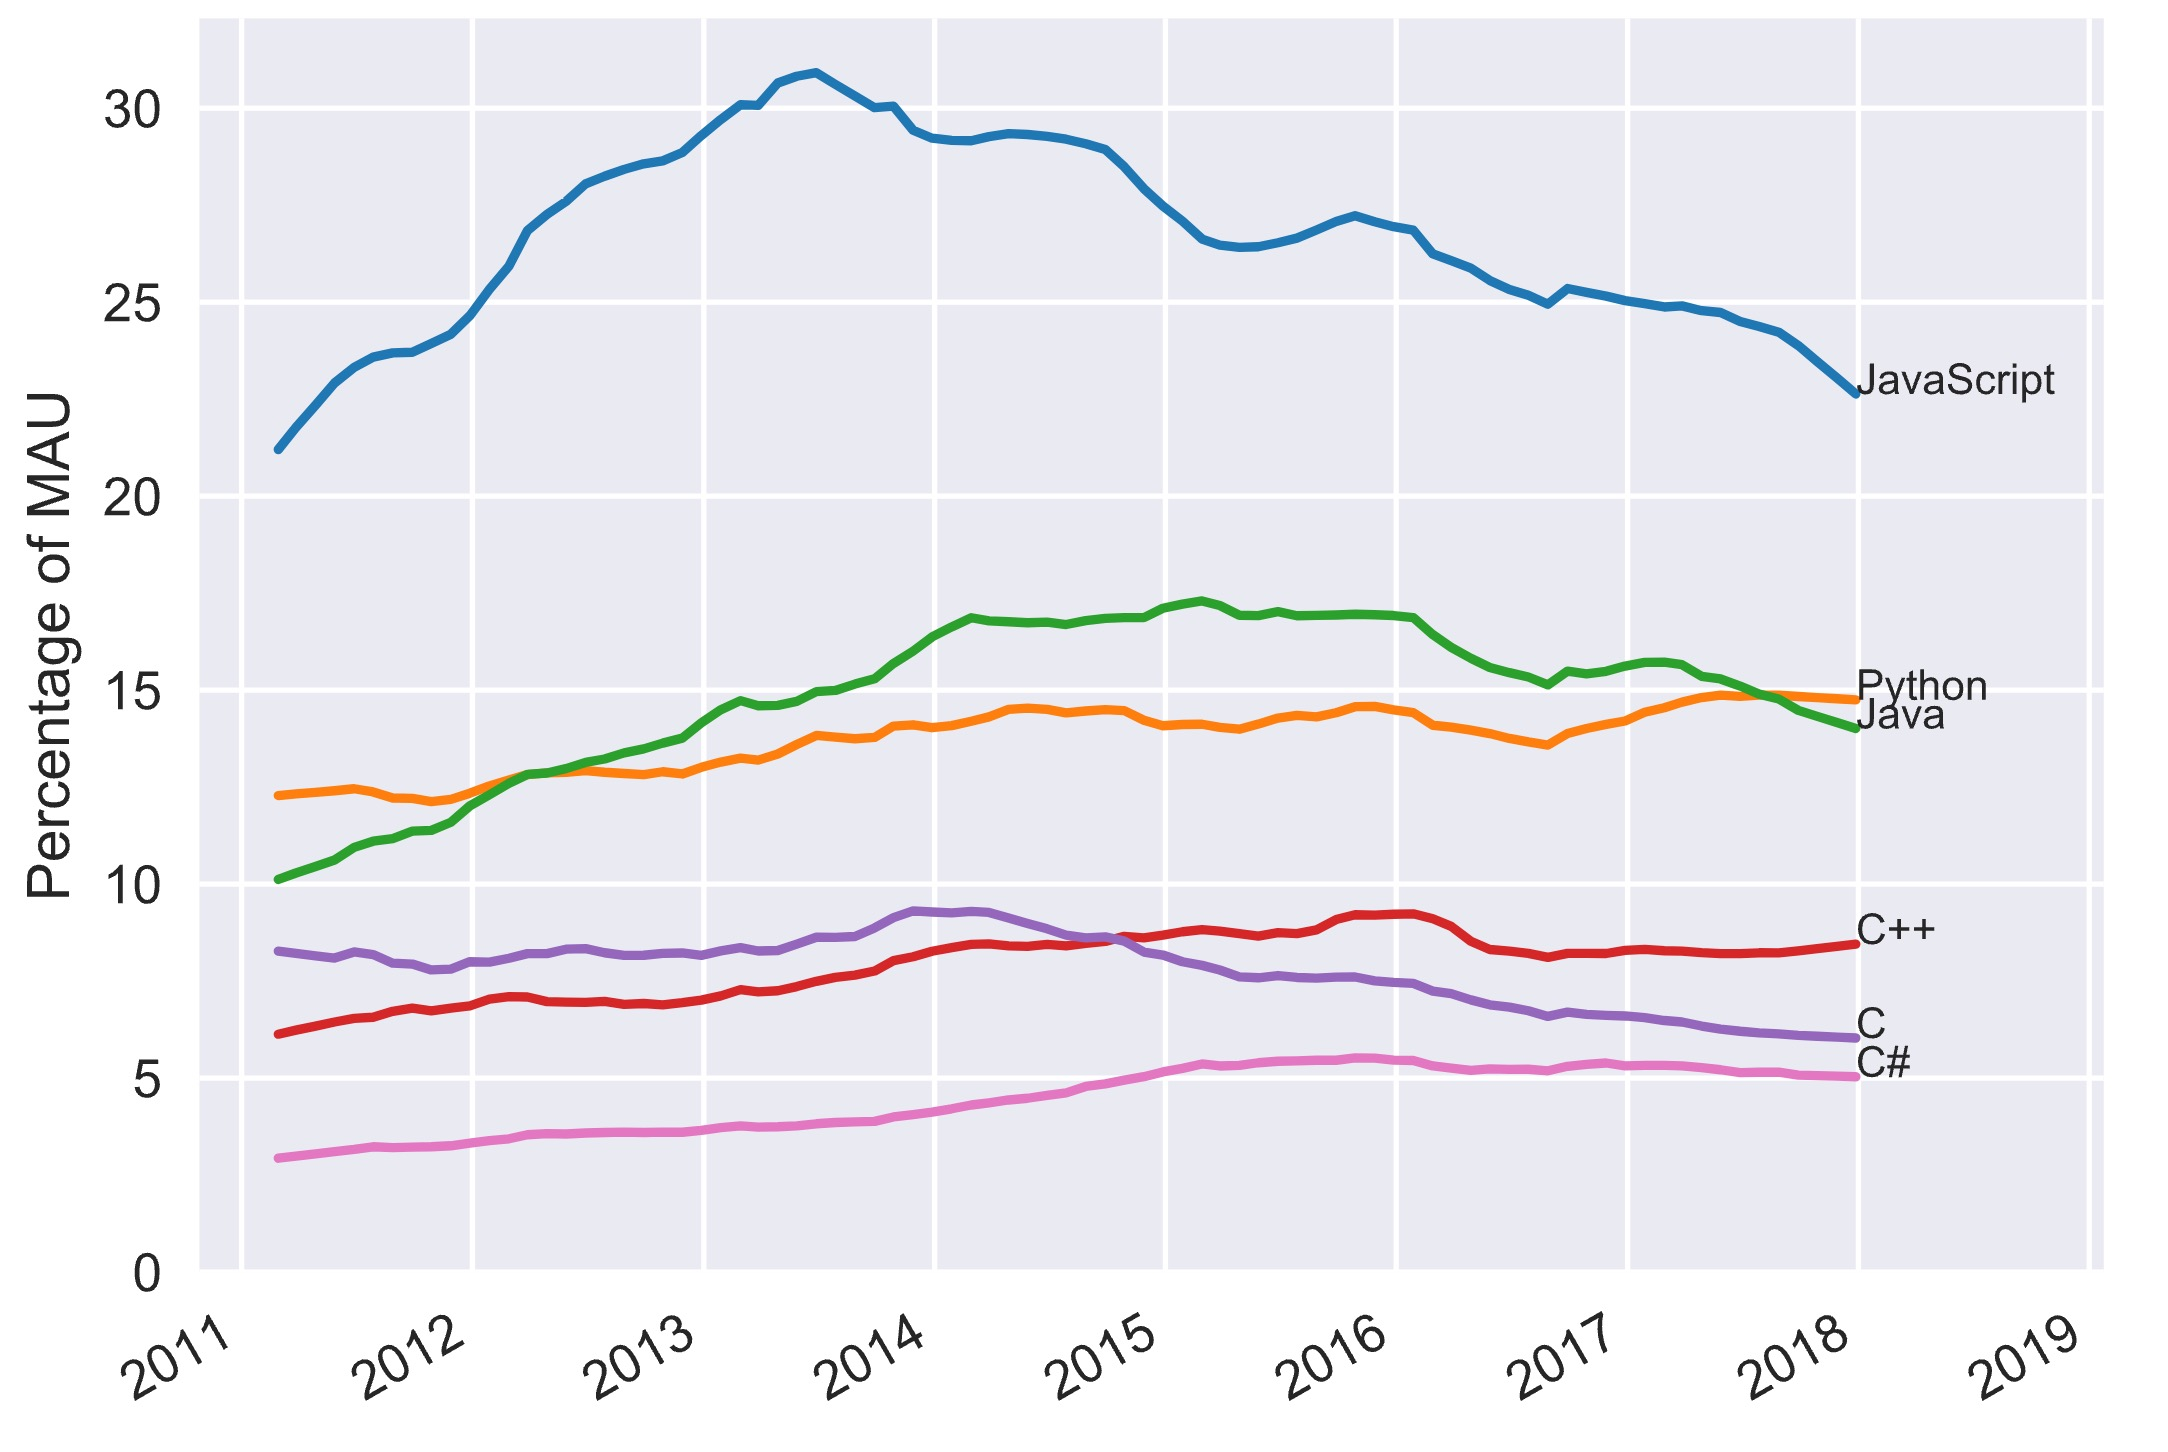
\includegraphics[width=.9\linewidth]{javascript_motivation.jpg}
    \caption{\url{https://www.benfrederickson.com}}
  \end{figure}
\end{frame}
% 6
\begin{frame}[fragile, t]
  \frametitle{JavaScript符号执行}
  什么是符号执行?
  \begin{figure}
    \centering
    \begin{minipage}[] {0.45\textwidth}
      \centering
      \begin{lstlisting}
        x = 'input'
        if(len(x) > 10){
          y = x
        } else {
          y = "error"
        }
      \end{lstlisting}
    \end{minipage}
    \hfill
    \begin{minipage}[] {0.45\textwidth}
      \centering
      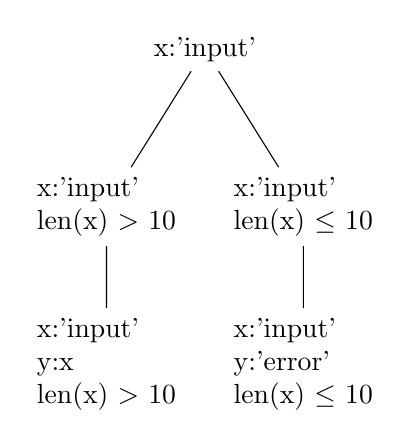
\begin{tikzpicture}[align=left, sibling distance=25mm, level distance=20mm]
        \node {x:'input'}
        child {node {x:'input'\\len(x) $>$ 10}
            child {node {x:'input'\\y:x\\len(x) $>$ 10}}
          }
        child {node {x:'input'\\len(x) $\leq$ 10}
            child {node {x:'input'\\y:'error'\\len(x) $\leq$ 10}}
          };
      \end{tikzpicture}
    \end{minipage}
  \end{figure}
\end{frame}

\begin{frame}[fragile, t]
  \frametitle{JavaScript符号执行}
  什么是符号执行?
  \begin{figure}
    \centering
    \begin{minipage}[] {0.45\textwidth}
      \centering
      \begin{lstlisting}
        x = 'input'
        if(len(x) > 10){
          y = x
        } else {
          y = "error"
        }
      \end{lstlisting}
    \end{minipage}
    \hfill
    \begin{minipage}[] {0.45\textwidth}
      \centering
      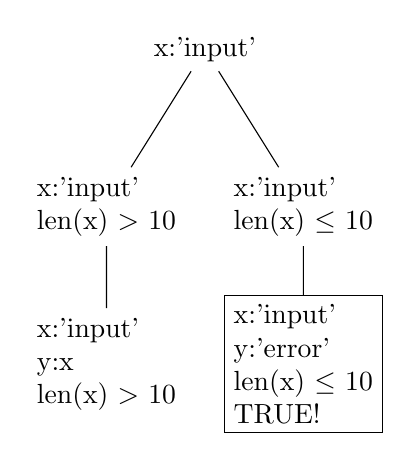
\begin{tikzpicture}[align=left, sibling distance=25mm, level distance=20mm]
        \node {x:'input'}
        child {node {x:'input'\\len(x) $>$ 10}
            child {node {x:'input'\\y:x\\len(x) $>$ 10}}
          }
        child {node {x:'input'\\len(x) $\leq$ 10}
            child {node[rectangle,draw] {x:'input'\\y:'error'\\len(x) $\leq$ 10\\TRUE!}}
          };
      \end{tikzpicture}
    \end{minipage}
  \end{figure}
\end{frame}

\begin{frame}[fragile, t]
  \frametitle{JavaScript符号执行}
  什么是符号执行?
  \begin{figure}
    \centering
    \begin{minipage}[] {0.45\textwidth}
      \centering
      \begin{lstlisting}
        x = 'input'
        if(len(x) > 10){
          y = x
        } else {
          y = "error"
        }
      \end{lstlisting}
    \end{minipage}
    \hfill
    \begin{minipage}[] {0.45\textwidth}
      \centering
      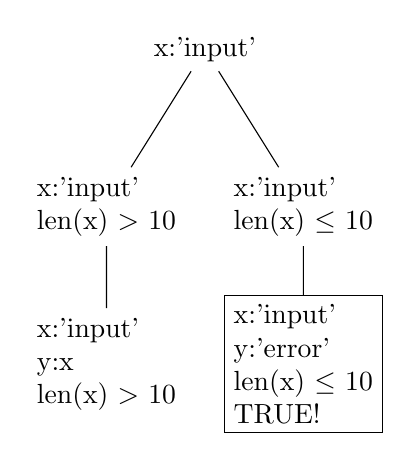
\begin{tikzpicture}[align=left, sibling distance=25mm, level distance=20mm]
        \node {x:'input'}
        child {node {x:'input'\\len(x) $>$ 10}
            child {node {x:'input'\\y:x\\len(x) $>$ 10}}
          }
        child {node {x:'input'\\len(x) $\leq$ 10}
            child {node[rectangle,draw] {x:'input'\\y:'error'\\len(x) $\leq$ 10\\TRUE!}}
          };
      \end{tikzpicture}
    \end{minipage}
  \end{figure}
  SMT求解器:$x="input"\wedge y="error"\wedge len(x)\leq 10$
\end{frame}

\section{国内外本学科领域的发展现状与趋势}
% 7
\begin{frame}[fragile, t]
  \frametitle{SMT官方文档}
  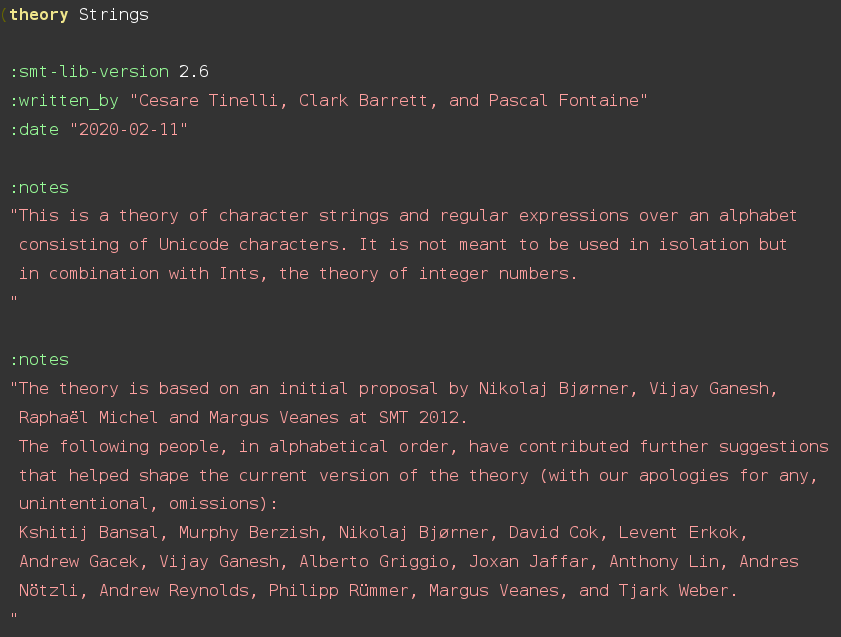
\includegraphics[width=\linewidth]{smtlib.png}
\end{frame}
% 8
\begin{frame}[fragile, t]
  \frametitle{字符串约束求解器}
  \begin{multicols}{2}
    \begin{itemize}
      \item Hampi
      \item Kaluza
      \item Stranger
      \item Gecode+S
      \item GStrings
      \item Z3-str/2/3/4
      \item CVC4/5
      \item Norn
      \item S3/p/\#
      \item Trau/+
      \item Sloth
      \item OSTRICH/+
      \item (MT-)ABC
      \item Woorpje
      \item BEK, REX
      \item SLOG, SLENT
      \item ...
    \end{itemize}
  \end{multicols}
\end{frame}
% 9
\begin{frame}
  \frametitle{JavaScript符号执行工具}
  \setstretch{1.5}
  \begin{multicols}{2}
    \begin{itemize}
      \item Kudzu/Kaluza
      \item Jalangi/2
      \item ExPoSE/2
      \item Aratha
      \item SAFE/$_str$
      \item SymJS
      \item leena
      \item extract-js
      \item ...
    \end{itemize}
  \end{multicols}
\end{frame}

\section{课题主要研究内容和目标}
% 10
\begin{frame}[fragile]
  \frametitle{课题主要研究内容和目标}
  \setstretch{1.5}
  \begin{itemize}
    \item 含整数数据类型的字符串约束求解技术
    \item 带有正则表达式捕获组的$\replaceall$函数的研究
    \item 对含有数组数据类型的字符串约束研究
    \item 字符串约束求解技术在JavaScript符号执行上的应用
  \end{itemize}
\end{frame}
% 11
\begin{frame}[fragile, t]
  \frametitle{含整数数据类型的字符串约束求解技术}
  \begin{block}{问题描述}
    输入的字符串约束中含有线性整数约束,含有带整数类型的字符串函数如$\indexof$函数、$\len$函数和$\substring$函数。
  \end{block}
\end{frame}

\begin{frame}[fragile, t]
  \frametitle{含整数数据类型的字符串约束求解技术}
  \begin{block}{问题描述}
    输入的字符串约束中含有线性整数约束,含有带整数类型的字符串函数如$\indexof$函数、$\len$函数和$\substring$函数。
  \end{block}
  \begin{align*}
    & \ x = "input" \\
    \wedge & \ \len(x) < 10\\
    \wedge &\ y = x\\
    \wedge &\ \indexof(y, "error") > 0\\
  \end{align*}
\end{frame}

\begin{frame}[fragile, t]
  \frametitle{含整数数据类型的字符串约束求解技术}
  \begin{block}{问题描述}
    输入的字符串约束中含有线性整数约束,含有带整数类型的字符串函数如$\indexof$函数、$\len$函数和$\substring$函数。
  \end{block}
  \begin{align*}
    & \ x = "input" \\
    \wedge & \ \len(x) < 10\\
    \wedge &\ y = x\\
    \wedge &\ \indexof(y, "error") > 0\\
  \end{align*}
  \begin{block}{研究内容和预期目标}
    开发能够处理整数数据类型的字符串约束求解器,能够处理上述字符串约束。同时和其他字符串约束求解器进行对比,验证其正确性和有效性。
  \end{block}
\end{frame}

%12
\begin{frame}[fragile, t]
  \frametitle{带有正则表达式捕获组的$\replaceall$函数的研究}
  \begin{block}{问题描述}
    输入的字符串约束中含有正则表达式捕获组,含有带正则表达式捕获组的字符串函数如$\replaceall$函数。
  \end{block}
\end{frame}

\begin{frame}[fragile, t]
  \frametitle{带有正则表达式捕获组的$\replaceall$函数的研究}
  \begin{block}{问题描述}
    输入的字符串约束中含有正则表达式捕获组,含有带正则表达式捕获组的字符串函数如$\replaceall$函数。
  \end{block}
  \begin{align*}
    & \ x = "input \ is\ right" \\
    \wedge &\ y = \extract(x, "(w+)\ is", 1)\\
    \wedge &\ y\not \in AttackPattern\\
  \end{align*}
\end{frame}

\begin{frame}[fragile, t]
  \frametitle{带有正则表达式捕获组的$\replaceall$函数的研究}
  \begin{block}{问题描述}
    输入的字符串约束中含有正则表达式捕获组,含有带正则表达式捕获组的字符串函数如$\replaceall$函数。
  \end{block}
  \begin{align*}
    & \ x = "input \ is\ right" \\
    \wedge &\ y = \extract(x, "(w+)\ is", 1)\\
    \wedge &\ y\not \in AttackPattern\\
  \end{align*}
  \begin{block}{研究内容和预期目标}
    开发能够处理正则表达式捕获组的字符串约束求解器,能够处理上述字符串约束。同时和其他字符串约束求解器进行对比,验证其正确性和有效性。
  \end{block}
\end{frame}

%13
\begin{frame}[fragile, t]
  \frametitle{对含有数组数据类型的字符串约束研究}
  \begin{block}{问题描述}
    输入的字符串约束中含有数组数据类型,含有带数组数据类型的字符串函数如$\mysplit$函数和$\myjoin$函数。
  \end{block}
\end{frame}

\begin{frame}[fragile, t]
  \frametitle{对含有数组数据类型的字符串约束研究}
  \begin{block}{问题描述}
    输入的字符串约束中含有数组数据类型,含有带数组数据类型的字符串函数如$\mysplit$函数和$\myjoin$函数。
  \end{block}
  \begin{align*}
    & \ x = "address?username=input" \\
    \wedge & \ a = \mysplit(x, "?")\\
    \wedge &\ y = a[1]\\
    \wedge &\ y \not \in AttackPattern\\
  \end{align*}
\end{frame}

\begin{frame}[fragile, t]
  \frametitle{对含有数组数据类型的字符串约束研究}
  \begin{block}{问题描述}
    输入的字符串约束中含有数组数据类型,含有带数组数据类型的字符串函数如$\mysplit$函数和$\myjoin$函数。
  \end{block}
  \begin{align*}
    & \ x = "address?username=input" \\
    \wedge & \ a = \mysplit(x, "?")\\
    \wedge &\ y = a[1]\\
    \wedge &\ y \not \in AttackPattern\\
  \end{align*}
  \begin{block}{研究内容和预期目标}
    开发能够处理数组数据类型的字符串约束求解器,能够处理上述字符串约束。同时和其他字符串约束求解器进行对比,验证其正确性和有效性。
  \end{block}
\end{frame}

%14
\begin{frame}[fragile, t]
  \frametitle{字符串约束求解技术在JavaScript符号执行上的应用}
  \begin{block}{问题描述}
    输入一段带有字符串函数的JavaScript代码,对其进行符号执行并生成路径约束,使用我们的字符串约束求解器进行求解,输出该代码的符号执行结果。
  \end{block}

\end{frame}

\begin{frame}[fragile, t]
  \frametitle{字符串约束求解技术在JavaScript符号执行上的应用}
  \begin{block}{问题描述}
    输入一段带有字符串函数的JavaScript代码,对其进行符号执行并生成路径约束,使用我们的字符串约束求解器进行求解,输出该代码的符号执行结果。
  \end{block}
  \begin{lstlisting}
    var x = goog.string.htmlEscape(name);
    var y = goog.string.escapeString(x);
    if(indexof(x, attack) > 0){
      alert("error");
    }
    nameElem.innerHTML =
    '<button onclick= "viewPerson(\' + y + '\')">' +
    x + '</button>';
  \end{lstlisting}

\end{frame}
\begin{frame}[fragile, t]
  \frametitle{字符串约束求解技术在JavaScript符号执行上的应用}
  \begin{block}{问题描述}
    输入一段带有字符串函数的JavaScript代码,对其进行符号执行并生成路径约束,使用我们的字符串约束求解器进行求解,输出该代码的符号执行结果。
  \end{block}
  \begin{lstlisting}
    var x = goog.string.htmlEscape(name);
    var y = goog.string.escapeString(x);
    if(indexof(x, attack) > 0){
      alert("error");
    }
    nameElem.innerHTML =
    '<button onclick= "viewPerson(\' + y + '\')">' +
    x + '</button>';
  \end{lstlisting}
  \begin{block}{研究内容和预期目标}
    开发能够处理JavaScript字符串约束的符号执行器,能够处理上述程序。同时和其他JavaScript符号执行工具进行对比,验证其正确性和有效性。
  \end{block}
\end{frame}

\section{拟采用的研究方法、技术路线及可行性分析}
%15
\begin{frame}
  \frametitle{字符串约束求解技术}
  在已有的字符串约束求解器OSTRICH上进行扩展。拟采用带有寄存器的自动机来处理带整数类型和数组类型的字符串约束,使用优先级流式字符串转换器来处理带有正则表达式捕获组的字符串约束。
  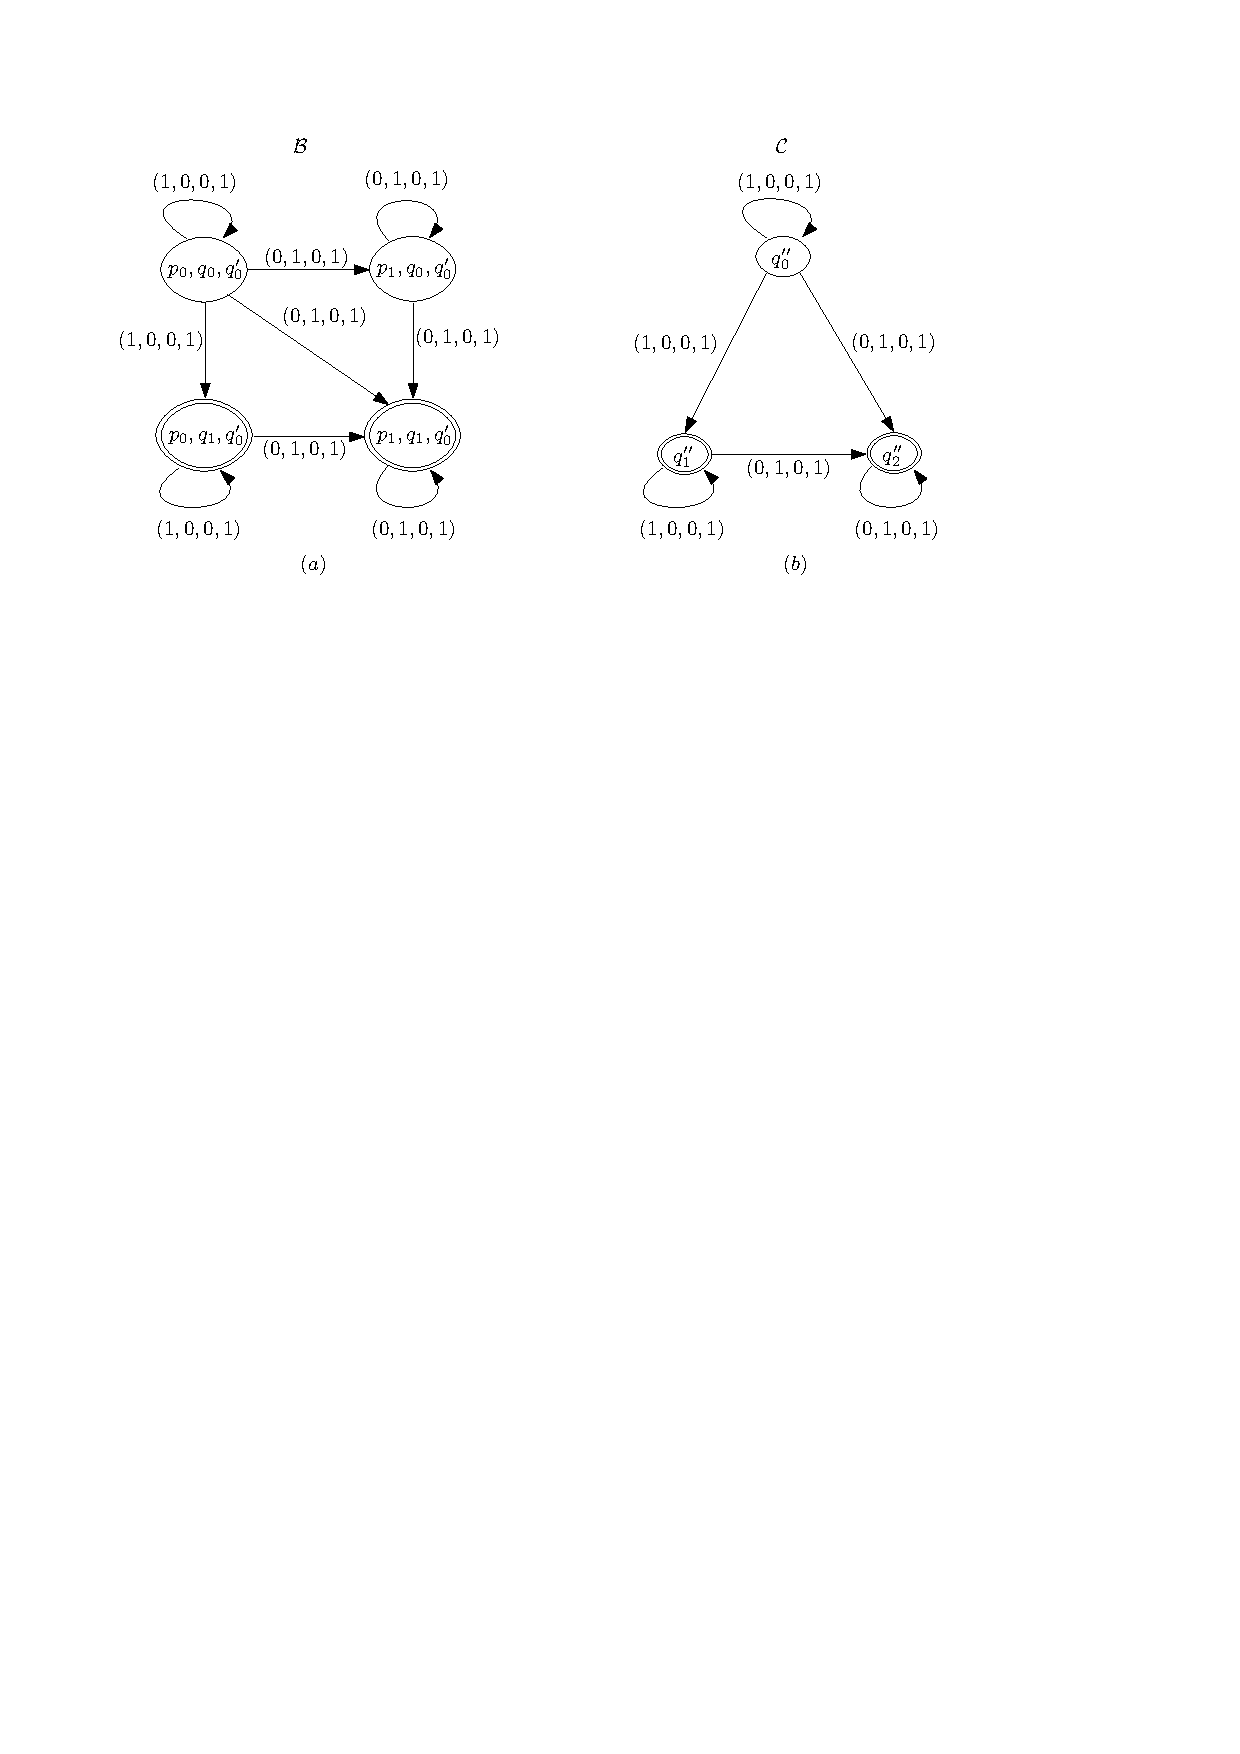
\includegraphics[width=\linewidth]{overview-cefa-reduced.pdf}
\end{frame}
%16 
\begin{frame}
  \frametitle{字符串约束求解技术在JavaScript符号执行上的应用}
  在已有的符号执行Aratha上进行扩展。拟对含有字符串函数的JavaScript代码进行符号执行,生成路径约束,使用我们的字符串约束求解器进行求解。使用Conclic执行技术,将符号执行和具体执行相结合,提高符号执行的效率。
  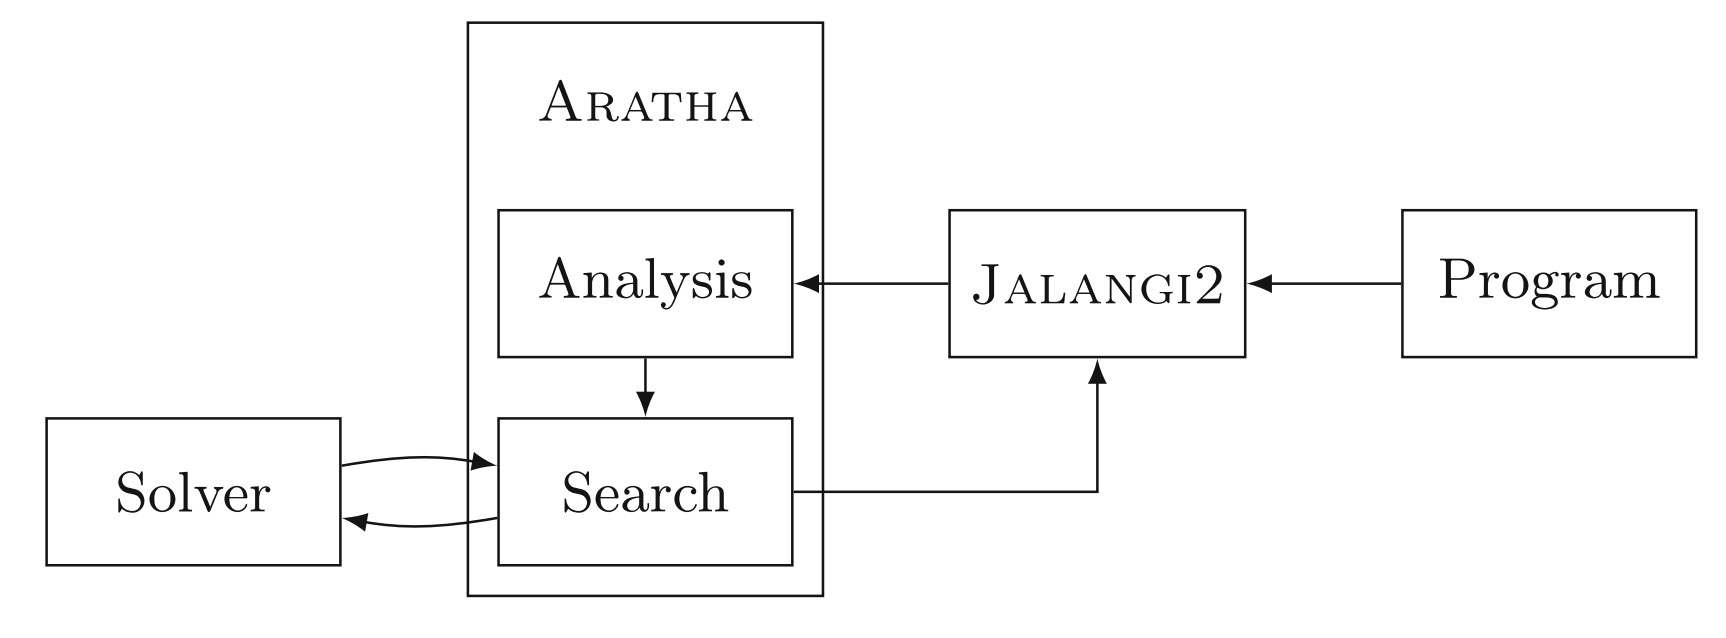
\includegraphics[width=\linewidth]{aratha}
\end{frame}
%17
\begin{frame}
  \frametitle{可行性分析}
  本课题有一定的研究基础,已经对字符串约束求解技术有了一定的了解,对字符串约束求解器OSTRICH和符号执行器Aratha有了一定的了解。已发表文章:
  \begin{itemize}
    \item T. Chen, M. Hague, J. He, \textbf{D. Hu}, A. Lin, P. Ruemmer, Z. Wu: A Decision Procedure for Path Feasibility of String Manipulating Programs with Integer Data Type. ATVA 2020
    \item P. Abdulla, M. Atig, Y. Chen, B. Diep, L. Holík, \textbf{D. Hu}, W. Tsai, Z. Wu, D. Yen: Solving Not-Substring Constraint with Flat Abstractionn. APLAS 2021.
    \item T. Chen, M. Hague, Z. Han, \textbf{D. Hu}, A. Lamas, A. Lin, S. Kan, P. Ruemmer, Z. Wu: Solving String Constraints With Regex-Dependent Functions Through Transducers With Priorities And Variables. POPL2022
  \end{itemize}
\end{frame}

\end{document}
